\documentclass[Orbiter User Manual.tex]{subfiles}
\begin{document}

\section{Flight recorder}
\label{sec:flight_rec}
You can record and play back your Orbiter simulation sessions with the built-in flight recorder feature. To open the recorder during a simulation, click record in the main menu (shortcut: \Ctrl\keystroke{F5}). Click the REC button to start the recording. Click STOP to turn the recorder off. A keyboard shortcut for starting and stopping the recording without opening the dialog is \Ctrl\keystroke{C}. Recording sessions are stored as new scenarios in the \textit{Playback} scenario folder. By default, they have the same name as the original scenario, but a different name can be specified in the dialog before starting the recorder. After a recording has been stopped, restarting the recorder will overwrite the earlier segment, unless a different name is chosen.\\
A running recording session is indicated by a blinking REC light in the top right corner.\\

\begin{figure}[H]
	\centering
	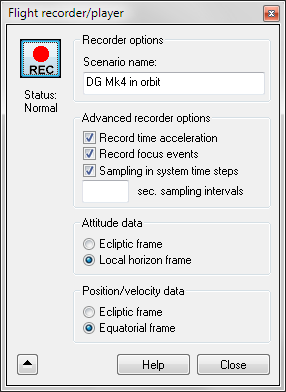
\includegraphics[width=0.4\hsize]{flight_recorder.png}
\end{figure}

\noindent
Some additional options can be accessed by pressing the $\blacktriangledown$ button in the dialog. These include

\begin{itemize}
\item \textbf{Record time acceleration:} Any changes in time acceleration during the session are recorded in the playback stream. During replay, the user has the option to set time compression automatically from the recorded data.
\item \textbf{Record focus events:} Switching the focus to a different spacecraft during the recording is recorded in the stream. The same switches will then occur in the playback.
\item \textbf{Sampling in system time steps:} If ticked, the intervals between recorded data samples are determined in system time, otherwise in simulation time. In system time, sampling is less dense during time compression. This allows to reduce the size of the data files when recording over long periods of time that are fast-forwarded during recording, but it can lead to noticeable position errors if the same time compression is not used during playback.
\item \textbf{Sampling intervals:} Not currently used.
\item \textbf{Attitude data:} The vessel attitude can be recorded either with respect to the global ecliptic frame of reference, or with respect to the local horizon of the current reference celestial body. This has no effect on the playback, but may be of interest if the data are used externally, e.g. for trajectory analysis.
\item \textbf{Position/velocity data:} Vessel position and velocity samples can be stored with respect to the ecliptic frame or the equatorial frame of the reference object. This has no effect on the playback, but may be of interest if the data are used externally, e.g. for trajectory analysis.
\end{itemize}

\noindent
To play back a previously recorded session, launch the scenario under the Playback scenario folder. During playback, all vessels will follow their pre-recorded trajectories and will not respond to manual user control. At the end of the playback the simulation will automatically switch back to manual mode, and the user can take over control. You can terminate the playback before the end of the data stream is reached by pressing \Ctrl\keystroke{C}. A running replay is indicated by a green playback symbol in the top right corder of the screen.\\
A playback is more powerful than just a video clip: the user still has various options to interact with the simulation. For example, it is possible to move the camera, change between cockpit and external views, and even manipulate the MFD instruments to access more fight data. You can however not manipulate the engines: all vessels follow their recorded trajectories.\\

\begin{figure}[H]
	\centering
	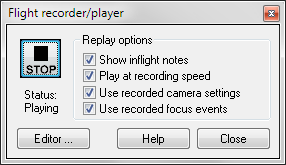
\includegraphics[width=0.4\hsize]{flight_recorder_playing.png}
\end{figure}

\noindent
Pressing \Ctrl\keystroke{F5} during a playback will open the Player dialog which can be used to stop playback and to set some playback options:

\begin{itemize}
\item \textbf{Show inflight notes:} Show/hide on-screen text embedded in the recording. Inflight notes can be added to recordings during post-processing, and are useful for creating demos and tutorials.
\item \textbf{Play at recording speed:} Use/ignore any time acceleration data stored in the recording. If this option is selected, time acceleration is applied from the recording stream, and manual time acceleration settings are disabled.
\item \textbf{Use recorded camera settings:} Recorded camera movements and cuts are applied in the playback. Turning off this option allows to operate the camera manually during playback.
\item \textbf{Use recorded focus events:} Any switches to different vessels are replicated in the playback. Turning off this option leaves the focus on the initial vessel.
\end{itemize}


\subsection{Trajectory and event data}
The data for recorded simulation sessions are stored under the Flights subdirectory. Orbiter creates a new subfolder for each recording, using the same name as the recorded scenario. Each vessel in the scenario writes three data streams to this folder, consisting of:

\begin{itemize}
\item \textbf{position and velocity} (*.pos). Contains a sequence of state vector samples, recorded relative to a reference planet, either in a non-rotating reference system (ecliptic and equinox of J2000.0), or a rotating equatorial reference system. As a result, trajectories are recorded in an absolute time frame. Samples are written in regular intervals (2 s) or if the velocity vector rotates by more than 5°.
\item \textbf{attitude} (*.att). Attitude data are saved as Euler angles of the spacecraft with respect to the ecliptic frame or local horizon frame. Samples are written whenever one of the angles has changed by more than a predefined threshold limit.
\item \textbf{Articulation events} (*.atc). This stream records changes in thrust levels of the spacecraft engines, and other event types (e.g. change of RCS mode, activation of autopilot functions, animations, etc.). It can also be used by custom vessel modules to store non-standard events. During playback, the vessel can retrieve these data to replicate the events.
\end{itemize}

\noindent
The recording folder also contains a system.dat file that holds global (non-vessel specific) events such as camera settings, time acceleration events and on-screen annotations and their timings. This system file can be modified and extended in post-processing with the \textit{Playback event editor} (see \ref{sec:flight_playbackedit}).\\
A complete recording session consists of the playback scenario in the Scenarios\textbackslash playback folder, and the corresponding flight data folder under the Flights directory. To share a playback with other Orbiter users, these files must be copied. Note that the scenario file can be moved to a different Scenario folder, but no two playback scenarios can have the same name.\\
Be aware that long simulation sessions (in particular during time acceleration) may lead to very large data files, if \textit{Sampling in system time steps} is disabled.\\
Not all 3$^{rd}$ party spacecraft add-ons may fully support the recorder/playback tool, if they implement non-standard features but do not support parsing these to/from the articulation stream.\\
Implementation details and flight recorder file format specifications can be found in "Orbiter Flight Recorder and Playback" in Orbiter Technical Reference.


\subsection{Playback event editor}
\label{sec:flight_playbackedit}
After recording a flight you have the option to enhance the playback with the use of the \textit{Playback editor}. You can

\begin{itemize}
\item add annotations which appear on the simulation window at particular times during the replay,
\item change camera positions,
\item modify the time compression settings applied during the playback.
\end{itemize}

\noindent
However, you cannot modify the recorded simulation itself (such as changing vessel trajectories, engine burn times, animations, etc.) To access the playback editor, start a previously recorded scenario, open the Player dialog box with \Ctrl\keystroke{F5}, and click the Editor button. This will open the playback editor dialog.\\
\\
\textbf{Event list}\\
The top part of the dialog box contains the \textit{event list} for the scenario. Initially, this may be empty, or contain some event tags that were inserted during the original recording.\\
Each line in the list represents an event. Each event contains

\begin{itemize}
\item a time stamp (simulation time from the start of the recording in seconds),
\item an event tag defining the event type,
\item any event type-specific parameters.
\end{itemize}

\noindent
The current position in the playback is indicated by a blinking line (<{}<{}<{}<). As the replay progresses, this marker is moving through the event list. Sometimes it may be useful to pause the playback (\Ctrl\keystroke{P} in the simulation window) to have more time to examine and edit the event list.\\
\\
\textbf{Adding a new event}\\
Events are always added at the current playback time (at the position of the <{}<{}<{}<{}< time marker). You can however later edit the time stamps of events to move them to a different position in the stream.

\begin{figure}[H]
	\centering
	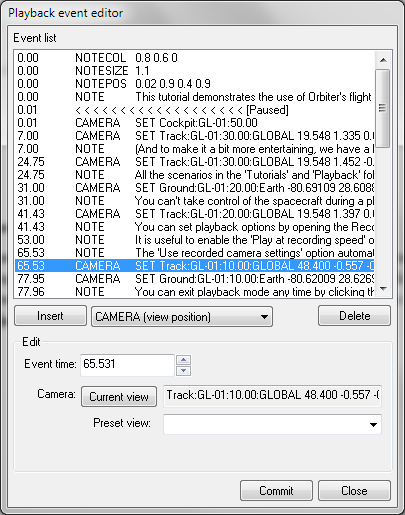
\includegraphics[width=0.4\hsize]{playback_editor.png}
\end{figure}

\noindent
First, select an event type from the drop-down list below the event list. The most important event types have entries in the list. For less frequently used items, pick the <Other> option and enter the event tag manually. After selecting a type, press the Insert button.\\
A new event line will appear in the list, and the Edit area in the lower part of the dialog box will allow to set any required parameters for the event.\\
\\
\textbf{Editing an existing event}\\
If you want to modify the parameters of an event already in the list, simply highlight it by clicking on a line in the list. The event parameters will appear in the Edit area, and you can modify them.\\
\\
\textbf{Deleting events}\\
To delete an event, highlight it by clicking on a line in the list. Then press the Delete button.\\
\\
\textbf{Committing changes}\\
To commit the changes you have made to the event list, press the Commit button at the bottom of the dialog box. This will save the modified event list in the playback file. Orbiter will immediately re-scan the file up to the current playback time so that any changes can be examined immediately.


\end{document}
